\section{Method}
This system provides interpolative playlist generation based on sets of data calculated for each song. The process begins by calculating ``characteristic elements'' \citep{Fingerhut2004} of the sound (or \emph{timbre}) known as features. Ideally, the extracted features become an absolute measure of the timbre of the song, such that two songs with similar features will sound similar. Next, the program reads these and generates a playlist by measuring the distance between the feature vectors.
%This similarity is biased according to a set of \emph{feature weights}, which are a measure of how important each feature is towards an overall accurate similarity metric.
%\citet{Pauws2002} states that ``if it is known that a set of songs is preferred (or fit a given context-of-use), then it is likely that preference can be generalised to other songs based solely on the fact that they are similar''.

Using GStreamer, libsndfile and FFTW3, audio data is read and the fourier transform computed, yielding data similar to that in figure \ref{fig:method:block}. Audio processing is done in three second blocks, with the mean, variance, skewness and kurtosis for each being stored in order to analyse the change in features over time. The order in which blocks are compared is of importance, so four different algorithms were implemented and evaluated for accuracy.

When a set of key tracks is given for playlist generation, the system loads in all known tracks, and compares similarity. The tracks are then ordered in the playlist to minimise overall distance between songs as best possible, while still adhering to the constraints set (no repeated artists, for example).
\begin{figure}[h]
	\centering
	\caption{A processing block from the beginning of \emph{Quick and to the Pointless} by \emph{Queens of the Stone Age}: It begins with ``Yeah yeah yeah yeah!'', the fourth ``yeah'' being overlaid with the entry of the guitar, with three claps towards the end.}
	\subfigure[Waveform (the signal read from the audio file)]{\label{fig:method:block:waveform}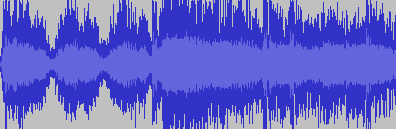
\includegraphics[width=0.5\textwidth]{method/waveform}}
	\subfigure[Spectrogram (a graphic representation of the spectrum returned by \software{FFTW3})]{\label{fig:method:block:spectrogram}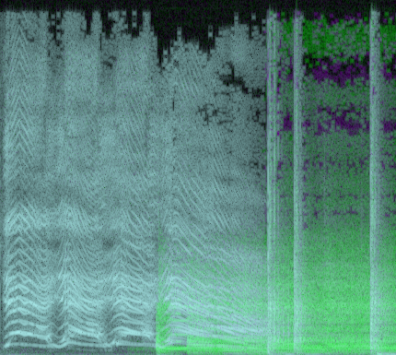
\includegraphics[width=0.5\textwidth]{method/spectrogram}}
	\label{fig:method:block}
\end{figure}

Feature extractors only work as a basic model to return statistics based on the timbre of the sound; it is therefore best to use a number of these models and let empirical evidence from testing `teach' the system which of these best represent measures which can determine the similarity of audio. The system includes a vector of weights for this purpose, training this will improve the accuracy of the system.

Training is done through analysis of a tester's answers to a \emph{music quiz}, which asks the tester to pick which two of three tracks played are the most similar. The results are then analysed, increasing the relevant weights according to features which were similar in the two tracks given. Training need only be done once, and it would be possible as a future development to also query existing symbolic systems such as \software{Last.fm} or \software{Ruffle} for similar tracks and use these for training.

The results from the music quiz can also be used in testing, to determine how well the system learns and how accurate the similarity measure is. When provided with the quiz results, the system adjusts weights aiming to return results more similar to the ones provided; using this, it is possible to automatically evaluate the efficacy of the system.

The overall design of the system meets the specification well; the intensive audio processing happens once and is stored, playlist generation then being a much less intensive (and hence faster) process. Data is summarised during processing, reducing the data storage (around 20KB per song) and subsequent processing time.

